\documentclass[11pt,a4paper]{article}

\usepackage[utf8]{inputenc}
\usepackage[T1]{fontenc}
\usepackage[english]{babel}
\usepackage{lmodern}
\usepackage[margin=2.4cm]{geometry}
\usepackage{booktabs}
\usepackage{longtable}
\usepackage{array}
\usepackage{amsmath}
\usepackage{siunitx}
\usepackage{eurosym}
\usepackage{graphicx}
\usepackage{xcolor}
\usepackage{caption}
\usepackage[hidelinks]{hyperref}

\sisetup{detect-weight=true, detect-family=true}

% Placeholder marker for numbers that still have to be pulled out of W&B.
\newcommand{\todo}[1]{\textcolor{red}{\textbf{[#1]}}}
\newcommand{\tbd}{\todo{TBD}}

\title{\textbf{Cultura Viva}\\[0.3em]
\large An on-device multimodal audio guide for Gaud\'i's Barcelona\\
\normalsize Model selection, benchmarks, and bill of materials}
\author{Cultura Viva team}
\date{13 September 2026}

\begin{document}
\maketitle

\begin{abstract}
\noindent
Cultura Viva is an interactive multimodal AI audio guide for Antoni Gaud\'i's
monuments in Barcelona --- Sagrada Fam\'ilia, Park G\"uell, Casa Mil\`a
(La Pedrera) and Casa Batll\'o --- running \emph{entirely on-device} on an
Arduino UNO Q. A visitor photographs an architectural element, asks a question
aloud, and hears a spoken answer in the guide personality they picked. No
network round-trip is involved at inference time.

This report documents the engineering work behind the device: the four-stage
pipeline (vision $\rightarrow$ speech-to-text $\rightarrow$ knowledge retrieval
$+$ small language model $\rightarrow$ speech synthesis), the comparative
benchmarks that selected each model under the board's memory and latency
budget, the latency optimisations that make the interaction feel immediate, and
the bill of materials with per-component prices.
\end{abstract}

\tableofcontents
\newpage

% ===========================================================================
\section{System overview}
% ===========================================================================

\subsection{Target platform}

The whole system runs on a single Arduino UNO Q, which is a dual-brain board:

\begin{itemize}
  \item \textbf{STM32 microcontroller (MCU).} Real-time C++ Arduino sketch
        driving the ST7735S LCD, the physical inputs (mode switch, action
        button, Modulino buttons/knob), the Modulino buzzer, GPS ingestion and
        minimap rendering.
  \item \textbf{Qualcomm QRB2210 Linux processor (MPU).} Quad-core ARM
        Cortex-A53 @ \SI{2.0}{\giga\hertz}, LPDDR4 RAM, \SI{32}{\giga\byte}
        eMMC, Debian Linux. Runs the Python AI pipeline: ONNX vision
        classification, faster-whisper STT, knowledge-graph retrieval, a
        quantised small language model via
        \texttt{llama-cpp-\discretionary{}{}{}python}, and Piper TTS.
\end{itemize}

The two halves talk over Arduino Bridge RPC. The board variant used for all
measurements reports \SI{3667}{\mega\byte} of usable RAM, i.e.\ the 4\,GB
model.

\subsection{The pipeline}

\begin{enumerate}
  \item \textbf{Capture \& validate.} The visitor frames a shot in camera mode
        (live view streamed to the LCD as Base64 RGB565 chunks over Bridge RPC)
        and presses the shutter. A per-monument ONNX classifier decides
        \emph{which architectural element} is in frame, or rejects the photo as
        off-distribution and asks for a retake.
  \item \textbf{Ask.} The visitor flips to map mode, picks a guide personality
        on the Modulino buttons (Artistic / Technical / Child), and records a
        spoken question. Recording ends by itself on silence.
  \item \textbf{Understand.} faster-whisper transcribes the question, biased
        towards the domain vocabulary (``Gaud\'i'', ``trencad\'is'',
        ``Sagrada Fam\'ilia'', \ldots) through an \texttt{initial\_prompt}.
  \item \textbf{Ground \& answer.} The recognised element ID indexes directly
        into a curated knowledge base (\texttt{knowledge\_base.json},
        \texttt{element\_sheets.json}), with keyword search as fallback. The
        retrieved facts plus the personality prompt plus the question go to the
        SLM.
  \item \textbf{Speak.} Piper synthesises the answer sentence by sentence,
        streamed to ALSA while the SLM is still decoding the next sentence.
        Volume tracks the Modulino knob live.
  \item \textbf{Map.} The visited landmark is marked on the LCD minimap, with
        position from the NEO-6M GPS.
\end{enumerate}

\subsection{Design constraints}

Every model choice in this report was made against the same budget:

\begin{center}
\begin{tabular}{lp{9.2cm}}
\toprule
\textbf{Constraint} & \textbf{Value} \\
\midrule
Compute            & 4$\times$ ARM Cortex-A53 @ \SI{2.0}{\giga\hertz}, CPU only \\
RAM for SLM weights + context & $<\SI{1.5}{\giga\byte}$ \\
SLM context window & 2048 tokens \\
Target response latency & $<\SI{3}{\second}$ to first audio \\
Connectivity at inference time & none (fully offline) \\
\bottomrule
\end{tabular}
\end{center}

There is no GPU backend: the \texttt{llama.cpp} build on the board is CPU-only,
and ONNX Runtime uses the CPU execution provider.

% ===========================================================================
\section{Vision models}
% ===========================================================================

\subsection{Problem formulation}

The vision stage answers ``\emph{what} is the visitor pointing at?''. It is a
per-monument classification problem, not a single global one: each monument has
its own set of architectural elements, so the label spaces are disjoint and a
shared classification head would be meaningless. We therefore train one
classifier per $(\text{monument}, \text{model})$ pair.

\begin{table}[h]
\centering
\caption{Element classes per monument. Class counts differ freely; nothing in
the pipeline assumes they match.}
\begin{tabular}{llp{7.6cm}}
\toprule
\textbf{Monument} & \textbf{$N$} & \textbf{Classes} \\
\midrule
Casa Batll\'o & 2 & \texttt{pla\_frontal}, \texttt{pla\_inferior} \\
Park G\"uell & 7 & \texttt{3\_viaductes}, \texttt{casa\_museu},
  \texttt{escalinata\_drac}, \texttt{pavellons\_consergeria},
  \texttt{placa\_natura}, \texttt{sala\_hipostila}, \texttt{turo\_3\_creus} \\
La Pedrera (Casa Mil\`a) & 3 & \texttt{facana\_1}, \texttt{facana\_2},
  \texttt{facana\_3} \\
Sagrada Fam\'ilia & 6 & \texttt{cupula}, \texttt{facana\_naixement},
  \texttt{facana\_passio}, \texttt{laterals}, \texttt{posterior},
  \texttt{torres} \\
\bottomrule
\end{tabular}
\end{table}

Classes are auto-detected from each monument's own subfolders in the dataset,
so adding a monument or a class requires no code change.

\subsection{Dataset and splits}

All images come from the \texttt{culturaviva/image\_1080} Hugging Face dataset,
one subfolder per monument. The split is fixed and shared by training,
validation and threshold calibration:

\begin{center}
\begin{tabular}{ll}
\toprule
Train / validation / test & 70\,\% / 15\,\% / 15\,\% \\
Split seed & 42 \\
Input resolution & $224 \times 224$ \\
Normalisation & mean $0.5$, std $0.5$ per channel \\
\bottomrule
\end{tabular}
\end{center}

Training and calibration both go through the same dataset loader, which
guarantees that OOD thresholds are calibrated on images the model was never fit
to.

\subsection{Backbones tried}

\begin{table}[h]
\centering
\caption{Vision backbones. A third backbone, ResNet-50
(\texttt{microsoft/resnet-50}), is present in the configuration but currently
commented out and was not part of the reported runs.}
\begin{tabular}{lll}
\toprule
\textbf{Name} & \textbf{Hugging Face checkpoint} & \textbf{Status} \\
\midrule
\texttt{mobilenetv2} & \texttt{google/mobilenet\_v2\_1.0\_224} & active \\
\texttt{vit}         & \texttt{google/vit-base-patch16-224}    & active \\
\texttt{resnet50}    & \texttt{microsoft/resnet-50}            & configured, disabled \\
\bottomrule
\end{tabular}
\end{table}

With 4 monuments $\times$ 2 active backbones, a full pass is \textbf{8 training
runs}. Each run gets its own dataset split instance, model instance, output
directory and Weights \& Biases run, named
\texttt{<monument>-<model>}, so runs never overwrite each other.

\paragraph{Training hyper-parameters.} Applied to every run unless a model
entry overrides them:

\begin{center}
\begin{tabular}{ll}
\toprule
Epochs & 8 \\
Batch size & 16 \\
Learning rate & $2\times10^{-5}$ \\
Model selection & best checkpoint by validation macro-F1 \\
\bottomrule
\end{tabular}
\end{center}

Evaluation reports \textbf{accuracy} and \textbf{macro-F1} (macro so that rare
elements are not drowned out by the frequent ones), computed on the held-out
test split at the end of each run.

\subsection{Results}

\begin{table}[h]
\centering
\caption{Test-split accuracy and macro-F1 per $(\text{monument},
\text{backbone})$ run. \emph{These values are logged to the Weights \& Biases
project} \texttt{cultura-viva} \emph{and were not exported into the repository;
the placeholders below are to be filled from the corresponding W\&B runs.}}
\label{tab:vision-results}
\begin{tabular}{llcccc}
\toprule
& & \multicolumn{2}{c}{\textbf{MobileNetV2}} & \multicolumn{2}{c}{\textbf{ViT-B/16}} \\
\cmidrule(lr){3-4}\cmidrule(lr){5-6}
\textbf{Monument} & \textbf{$N$} & Acc. & macro-F1 & Acc. & macro-F1 \\
\midrule
Casa Batll\'o            & 2 & \tbd & \tbd & \tbd & \tbd \\
Park G\"uell             & 7 & \tbd & \tbd & \tbd & \tbd \\
La Pedrera (Casa Mil\`a) & 3 & \tbd & \tbd & \tbd & \tbd \\
Sagrada Fam\'ilia        & 6 & \tbd & \tbd & \tbd & \tbd \\
\midrule
\textbf{Mean}            &   & \tbd & \tbd & \tbd & \tbd \\
\bottomrule
\end{tabular}
\end{table}

\paragraph{What ships.} Two exported classifiers are currently deployed on the
device, under \texttt{models/\discretionary{}{}{}vision/\discretionary{}{}{}<location>/}: Park G\"uell (7 element
classes $+$ \texttt{unknown}) and Sagrada Fam\'ilia (6 element classes $+$
\texttt{unknown}). Each is a \texttt{model.onnx} plus a \texttt{labels.json}
carrying the label map, input size and normalisation constants, so the
board-side code needs no per-model configuration.

\subsection{Out-of-distribution rejection}

A real visitor will point the camera at a tree, another tourist, or the sky. A
plain \texttt{argmax} classifier is obliged to name an architectural element
anyway, which would produce a confident, grounded, entirely wrong audio guide
answer. The pipeline therefore puts a gate in front of the prediction. The
input is rejected as \texttt{not\_sure} when \emph{either} signal fires:

\begin{align}
H(p) = -\sum_{i=1}^{N} p_i \ln p_i \;&>\; \tau_{H}
  &&\text{(predictive entropy too high)}\\[0.2em]
\max_i p_i \;&<\; \tau_{\text{conf}}
  &&\text{(peak confidence too low)}
\end{align}

Defaults are $\tau_{H} = 0.5 \ln N$ --- auto-scaled to each monument's class
count, so a 2-class and a 7-class head are held to comparable standards --- and
$\tau_{\text{conf}} = 0.50$.

Thresholds merge across three levels, \emph{global $\rightarrow$ monument
$\rightarrow$ model}, with an optional CLI override on top; the most specific
setting wins. This matters because the backbones do not calibrate alike:
MobileNetV2 tends to run less confident than ViT, and can be loosened on its own
without touching the other heads.

\texttt{calibrate\_thresholds.py} sweeps the validation split and suggests
$(\tau_{H}, \tau_{\text{conf}})$ for a given checkpoint, subject to a
\emph{recall target} --- how much in-distribution recall must be preserved,
default 95\,\%. It prints a ready-to-paste YAML snippet.

\subsection{Export path}

\begin{enumerate}
  \item \texttt{train\_classifier.py} --- fine-tunes every
        $(\text{monument}, \text{model})$ combination in \texttt{config.yaml}.
  \item \texttt{export\_to\_onnx.py} --- converts one fine-tuned checkpoint
        into \texttt{model.onnx} $+$ \texttt{labels.json}.
  \item \texttt{calibrate\_thresholds.py} --- suggests the OOD thresholds.
  \item \texttt{inference.py} --- runs an exported checkpoint on a single image
        with the gate applied; also importable as \texttt{MonumentClassifier},
        which is how the device uses it.
\end{enumerate}

% ===========================================================================
\section{Benchmarks}
% ===========================================================================

Three separate benchmark suites were built, one per non-vision stage. All three
target the same hardware; where a measurement was taken on a host PC rather
than on the board, this is stated explicitly.

% ---------------------------------------------------------------------------
\subsection{Small language model}
% ---------------------------------------------------------------------------

\subsubsection{Candidates}

Five instruction-tuned small models were evaluated, all at \texttt{Q4\_K\_M}
quantisation so that weights plus a 2k context fit the
$<\SI{1.5}{\giga\byte}$ budget.

\begin{table}[h]
\centering
\caption{SLM candidates. RAM footprint is weights plus 2k context.}
\begin{tabular}{llrr}
\toprule
\textbf{Model} & \textbf{Ollama tag} & \textbf{Weights} & \textbf{RAM} \\
\midrule
Qwen 2.5 1.5B Instruct  & \texttt{qwen2.5:1.5b} & \SI{1.10}{\giga\byte} & \SI{1.45}{\giga\byte} \\
Llama 3.2 1B Instruct   & \texttt{llama3.2:1b}  & \SI{0.80}{\giga\byte} & \SI{1.10}{\giga\byte} \\
Gemma 3 1B IT           & \texttt{gemma3:1b}    & \SI{0.85}{\giga\byte} & \SI{1.15}{\giga\byte} \\
SmolLM2 1.7B Instruct   & \texttt{smollm2:1.7b} & \SI{1.15}{\giga\byte} & \SI{1.50}{\giga\byte} \\
Qwen 2.5 0.5B Instruct  & \texttt{qwen2.5:0.5b} & \SI{0.39}{\giga\byte} & \SI{0.65}{\giga\byte} \\
\bottomrule
\end{tabular}
\end{table}

\subsubsection{Protocol}

\begin{itemize}
  \item \textbf{Test set.} 38 curated Gaud\'i questions with reference answers
        and retrieved contexts (\texttt{eval/testset.json}).
  \item \textbf{Generation.} \texttt{temperature} $=0.1$,
        \texttt{max\_tokens} $=128$, context window 2048, 4 threads,
        batch size 256.
  \item \textbf{Judge.} Ragas, scoring \emph{Faithfulness},
        \emph{AnswerRelevancy}, \emph{ContextPrecision} and
        \emph{ContextRecall}, driven by a \emph{local} Ollama judge
        (\texttt{qwen2.5:7b}, temperature $0$) with
        \texttt{all-MiniLM-L6-v2} sentence embeddings. Keeping the judge local
        means the evaluation is reproducible offline and no test data leaves
        the machine.
  \item \textbf{On-device re-run.} \texttt{benchmark\_arduino.py} re-runs the
        same 38 questions on the Cortex-A53 through
        \texttt{llama-cpp-python} built with
        \texttt{-march=armv8-a -mtune=cortex-a53}, and the resulting
        predictions are scored with the same Ragas judge back on the PC.
\end{itemize}

\subsubsection{Results}

\begin{table}[h]
\centering
\caption{Per-answer generation wall-clock over the 38-question test set, as
recorded in the checked-in prediction files. These runs were produced through
Ollama on the development host; they are \emph{not} Cortex-A53 timings and
should be read as a relative ordering between candidates, not as device
latency.}
\begin{tabular}{lrrrr}
\toprule
\textbf{Model} & \textbf{Mean (s)} & \textbf{Median (s)} & \textbf{Min (s)} & \textbf{Max (s)} \\
\midrule
Llama 3.2 1B Instruct  & 2.42 & 2.40 & 2.10 & 4.33 \\
Qwen 2.5 0.5B Instruct & 2.43 & 2.41 & 2.09 & 3.59 \\
Gemma 3 1B IT          & 2.57 & 2.48 & 2.17 & 5.52 \\
Qwen 2.5 1.5B Instruct & 2.61 & 2.61 & 2.14 & 4.97 \\
SmolLM2 1.7B Instruct  & 2.79 & 2.65 & 2.18 & 5.96 \\
\bottomrule
\end{tabular}
\end{table}

The spread in generation time is small --- roughly 15\,\% between the fastest
and the slowest candidate --- which is the important negative result: on this
workload, \emph{latency does not discriminate between the candidates}, so the
choice can be made on answer quality and memory headroom instead.

\begin{table}[h]
\centering
\caption{Ragas scores over the 38-question test set. \emph{The scored results
(\texttt{eval/results/}) are not checked into the repository; re-run
\texttt{main.py benchmark} to regenerate.}}
\begin{tabular}{lcccc}
\toprule
\textbf{Model} & \textbf{Faithful.} & \textbf{Ans.\ Rel.} & \textbf{Ctx.\ Prec.} & \textbf{Ctx.\ Rec.} \\
\midrule
Qwen 2.5 1.5B Instruct  & \tbd & \tbd & \tbd & \tbd \\
Llama 3.2 1B Instruct   & \tbd & \tbd & \tbd & \tbd \\
Gemma 3 1B IT           & \tbd & \tbd & \tbd & \tbd \\
SmolLM2 1.7B Instruct   & \tbd & \tbd & \tbd & \tbd \\
Qwen 2.5 0.5B Instruct  & \tbd & \tbd & \tbd & \tbd \\
\bottomrule
\end{tabular}
\end{table}

\paragraph{Selected.} \textbf{Qwen 2.5 1.5B Instruct}, \texttt{Q4\_K\_M}
(\texttt{qwen2.5-1.5b-instruct-q4\_k\_m.gguf}), is the configured default for
Arduino deployment. Qwen 2.5 0.5B remains a supported fallback for the 2\,GB
board variant, where the 1.5B model's \SI{1.45}{\giga\byte} working set is
uncomfortably tight.

% ---------------------------------------------------------------------------
\subsection{Speech-to-text}
% ---------------------------------------------------------------------------

\subsubsection{Engines compared}

\begin{table}[h]
\centering
\caption{STT engines evaluated, all on the Whisper Base model family.}
\begin{tabular}{lll}
\toprule
\textbf{Engine} & \textbf{Runtime} & \textbf{Status} \\
\midrule
\texttt{faster-whisper} & CTranslate2, INT8 quantisation & primary \\
\texttt{whisper.cpp}    & native C++ / GGML, ARM NEON SIMD & primary \\
\texttt{vosk}           & Kaldi-derived & optional \\
\texttt{sherpa-onnx}    & ONNX Runtime & optional \\
\bottomrule
\end{tabular}
\end{table}

For \texttt{whisper.cpp}, \texttt{pywhispercpp}'s bundled backend is rebuilt
against the target core:

\begin{quote}\ttfamily\small
export CFLAGS="-O3 -mcpu=cortex-a53"\\
export CXXFLAGS="-O3 -mcpu=cortex-a53"\\
uv pip install --force-reinstall pywhispercpp>=1.2.0
\end{quote}

On 64-bit aarch64 NEON is on by default; \texttt{-mcpu=cortex-a53} is about
instruction scheduling for this specific core.

\subsubsection{Metrics and optimisations}

The harness measures \textbf{WER}, \textbf{CER}, \textbf{keyword-spotting
accuracy}, \textbf{real-time factor} (inference time / audio duration) and
\textbf{peak RAM}.

Keyword-spotting accuracy deserves a note. A generic WER number hides the
failure that actually matters for an audio guide: a transcript that gets
``Gaud\'i'', ``trencad\'is'' or ``Sagrada Fam\'ilia'' wrong will retrieve the
wrong knowledge sheet, and the whole answer is then confidently off-topic. The
decoder is therefore biased towards the domain vocabulary through an
\texttt{initial\_prompt}:

\begin{quote}\itshape\small
Cultura Viva audio guide in Barcelona about Antoni Gaud\'i, Sagrada Fam\'ilia
basilica, Nativity, Passion, and Glory facades, Catalan modernisme
architecture, Casa Batll\'o, Casa Mil\`a, Park G\"uell, dragon and salamander
sculptures, and trencad\'is mosaics.
\end{quote}

For \texttt{faster-whisper} the same terms are additionally passed as explicit
\texttt{hotwords}. Further tuning:

\begin{itemize}
  \item \textbf{4 CPU threads} --- the QRB2210 has exactly 4 Cortex-A53 cores,
        so 4 saturates the CPU without paying context-switch overhead.
  \item \textbf{INT8 compute type} --- keeps the model comfortably inside
        LPDDR4 and maximises memory bandwidth.
  \item \textbf{Greedy decoding} --- \texttt{temperature} $=0.0$,
        \texttt{beam\_size} $=1$, to minimise RTF.
\end{itemize}

\subsubsection{Results}

The evaluation set is \textbf{24 synthetic visitor utterances}, varied across
register (neutral, polite, child-like), intent (materials, history, \ldots) and
speaker voice, with controlled background noise, each annotated with its target
keywords.

\begin{table}[h]
\centering
\caption{STT results over the 24-utterance set, domain bias applied. Timings
are from the \texttt{results\_computer/} run. \emph{Only
\texttt{faster-whisper:base.en} results are checked into the repository; the
remaining engines' rows are to be filled from a re-run.}}
\small
\begin{tabular}{lrrrrr}
\toprule
\textbf{Engine} & \textbf{WER} & \textbf{CER} & \textbf{Keyword acc.} & \textbf{Peak RAM} & \textbf{Model} \\
\midrule
\texttt{faster-whisper:base.en} & 0.164 & 0.093 & 96.1\,\% & \SI{397}{\mega\byte} & \SI{141}{\mega\byte} \\
\texttt{whisper.cpp:base.en-q5\_1} & \tbd & \tbd & \tbd & \tbd & \tbd \\
\texttt{vosk} & \tbd & \tbd & \tbd & \tbd & \tbd \\
\texttt{sherpa-onnx} & \tbd & \tbd & \tbd & \tbd & \tbd \\
\bottomrule
\end{tabular}
\end{table}

A \SI{16.4}{\percent} word error rate alongside \SI{96.1}{\percent} keyword
accuracy is exactly the shape we were optimising for: the transcript is
imperfect in its function words but almost never wrong about the proper nouns
that drive retrieval.

\paragraph{Selected.} \textbf{faster-whisper} with the \texttt{base.en} model
at INT8, which is what the device ships
(\texttt{models/stt/faster-whisper-base.en}).

% ---------------------------------------------------------------------------
\subsection{Text-to-speech}
% ---------------------------------------------------------------------------

\subsubsection{Candidates}

18 ONNX voices are registered in \texttt{models\_config.json}: three VITS
models exported from Hugging Face (MMS-TTS English, VITS LJSpeech, VITS VCTK)
and 15 Piper voices (Lessac, Ryan, Amy, Alan, Cori, each in low / medium / high
quality). 15 of the 18 were actually timed; \texttt{piper-amy-high},
\texttt{piper-alan-high} and \texttt{piper-cori-low} were not run.

Audio quality is explicitly out of scope for this benchmark --- it measures
\emph{inference time and footprint only}. Voice character was chosen separately,
by ear, per guide personality.

\subsubsection{Protocol}

Measured on the UNO Q itself (Qualcomm QRB2210, Cortex-A53, 4 threads,
\SI{3667}{\mega\byte} RAM detected), 2026-08-26. Each model is loaded once,
given 1 untimed warm-up run, then timed over \textbf{9 runs} round-robin
balanced across sentence-length buckets --- short ($\le$ 8 words), medium
(9--16), long ($\ge$ 17) --- drawn from a fixed set of Gaud\'i sentences.

\begin{table}[h]
\centering
\caption{TTS inference time on the Arduino UNO Q. Median seconds per sentence
by length bucket; RTF is the median of (inference time / generated audio
duration), so $\text{RTF} < 1$ means the voice synthesises faster than
real time. Disk size is the configured on-disk model size.}
\label{tab:tts}
\small
\begin{tabular}{lrrrrr}
\toprule
\textbf{Voice} & \textbf{Disk (MB)} & \textbf{Short (s)} & \textbf{Medium (s)} & \textbf{Long (s)} & \textbf{RTF} \\
\midrule
\multicolumn{6}{l}{\emph{VITS (ONNX Runtime, CPU)}} \\
MMS-TTS (English, VITS, ONNX) & 138 & 12.91 & 21.95 & 40.92 & 3.88 \\
VITS (LJSpeech, ONNX) & 332 & 15.39 & 43.89 & 59.04 & 3.78 \\
VITS (VCTK, multi-speaker, ONNX) & 150 & 13.69 & 34.43 & 49.50 & 3.80 \\
\midrule
\multicolumn{6}{l}{\emph{Piper}} \\
Piper (en\_US-lessac-low) & 20 & 1.61 & 4.12 & 6.00 & 0.62 \\
Piper (en\_US-lessac-medium) & 63 & 1.91 & 4.91 & 7.28 & 0.77 \\
Piper (en\_US-lessac-high) & 113 & 12.86 & 33.82 & 50.45 & 5.19 \\
Piper (en\_US-ryan-low) & 20 & 1.57 & 3.89 & 5.87 & 0.63 \\
Piper (en\_US-ryan-medium) & 63 & 1.94 & 5.36 & 7.43 & 0.80 \\
Piper (en\_US-ryan-high) & 113 & 12.52 & 37.24 & 51.76 & 5.31 \\
Piper (en\_US-amy-low) & 20 & 1.79 & 4.28 & 5.95 & 0.61 \\
Piper (en\_US-amy-medium) & 63 & 2.44 & 5.83 & 8.23 & 0.80 \\
Piper (en\_GB-alan-low) & 20 & 1.85 & 5.07 & 7.30 & 0.64 \\
Piper (en\_GB-alan-medium) & 63 & 2.39 & 6.14 & 8.67 & 0.75 \\
Piper (en\_GB-cori-medium) & 63 & 2.27 & 4.51 & 7.19 & 0.81 \\
Piper (en\_GB-cori-high) & 113 & 13.31 & 31.94 & 52.32 & 5.27 \\
\bottomrule
\end{tabular}
\end{table}

\begin{figure}[h]
\centering
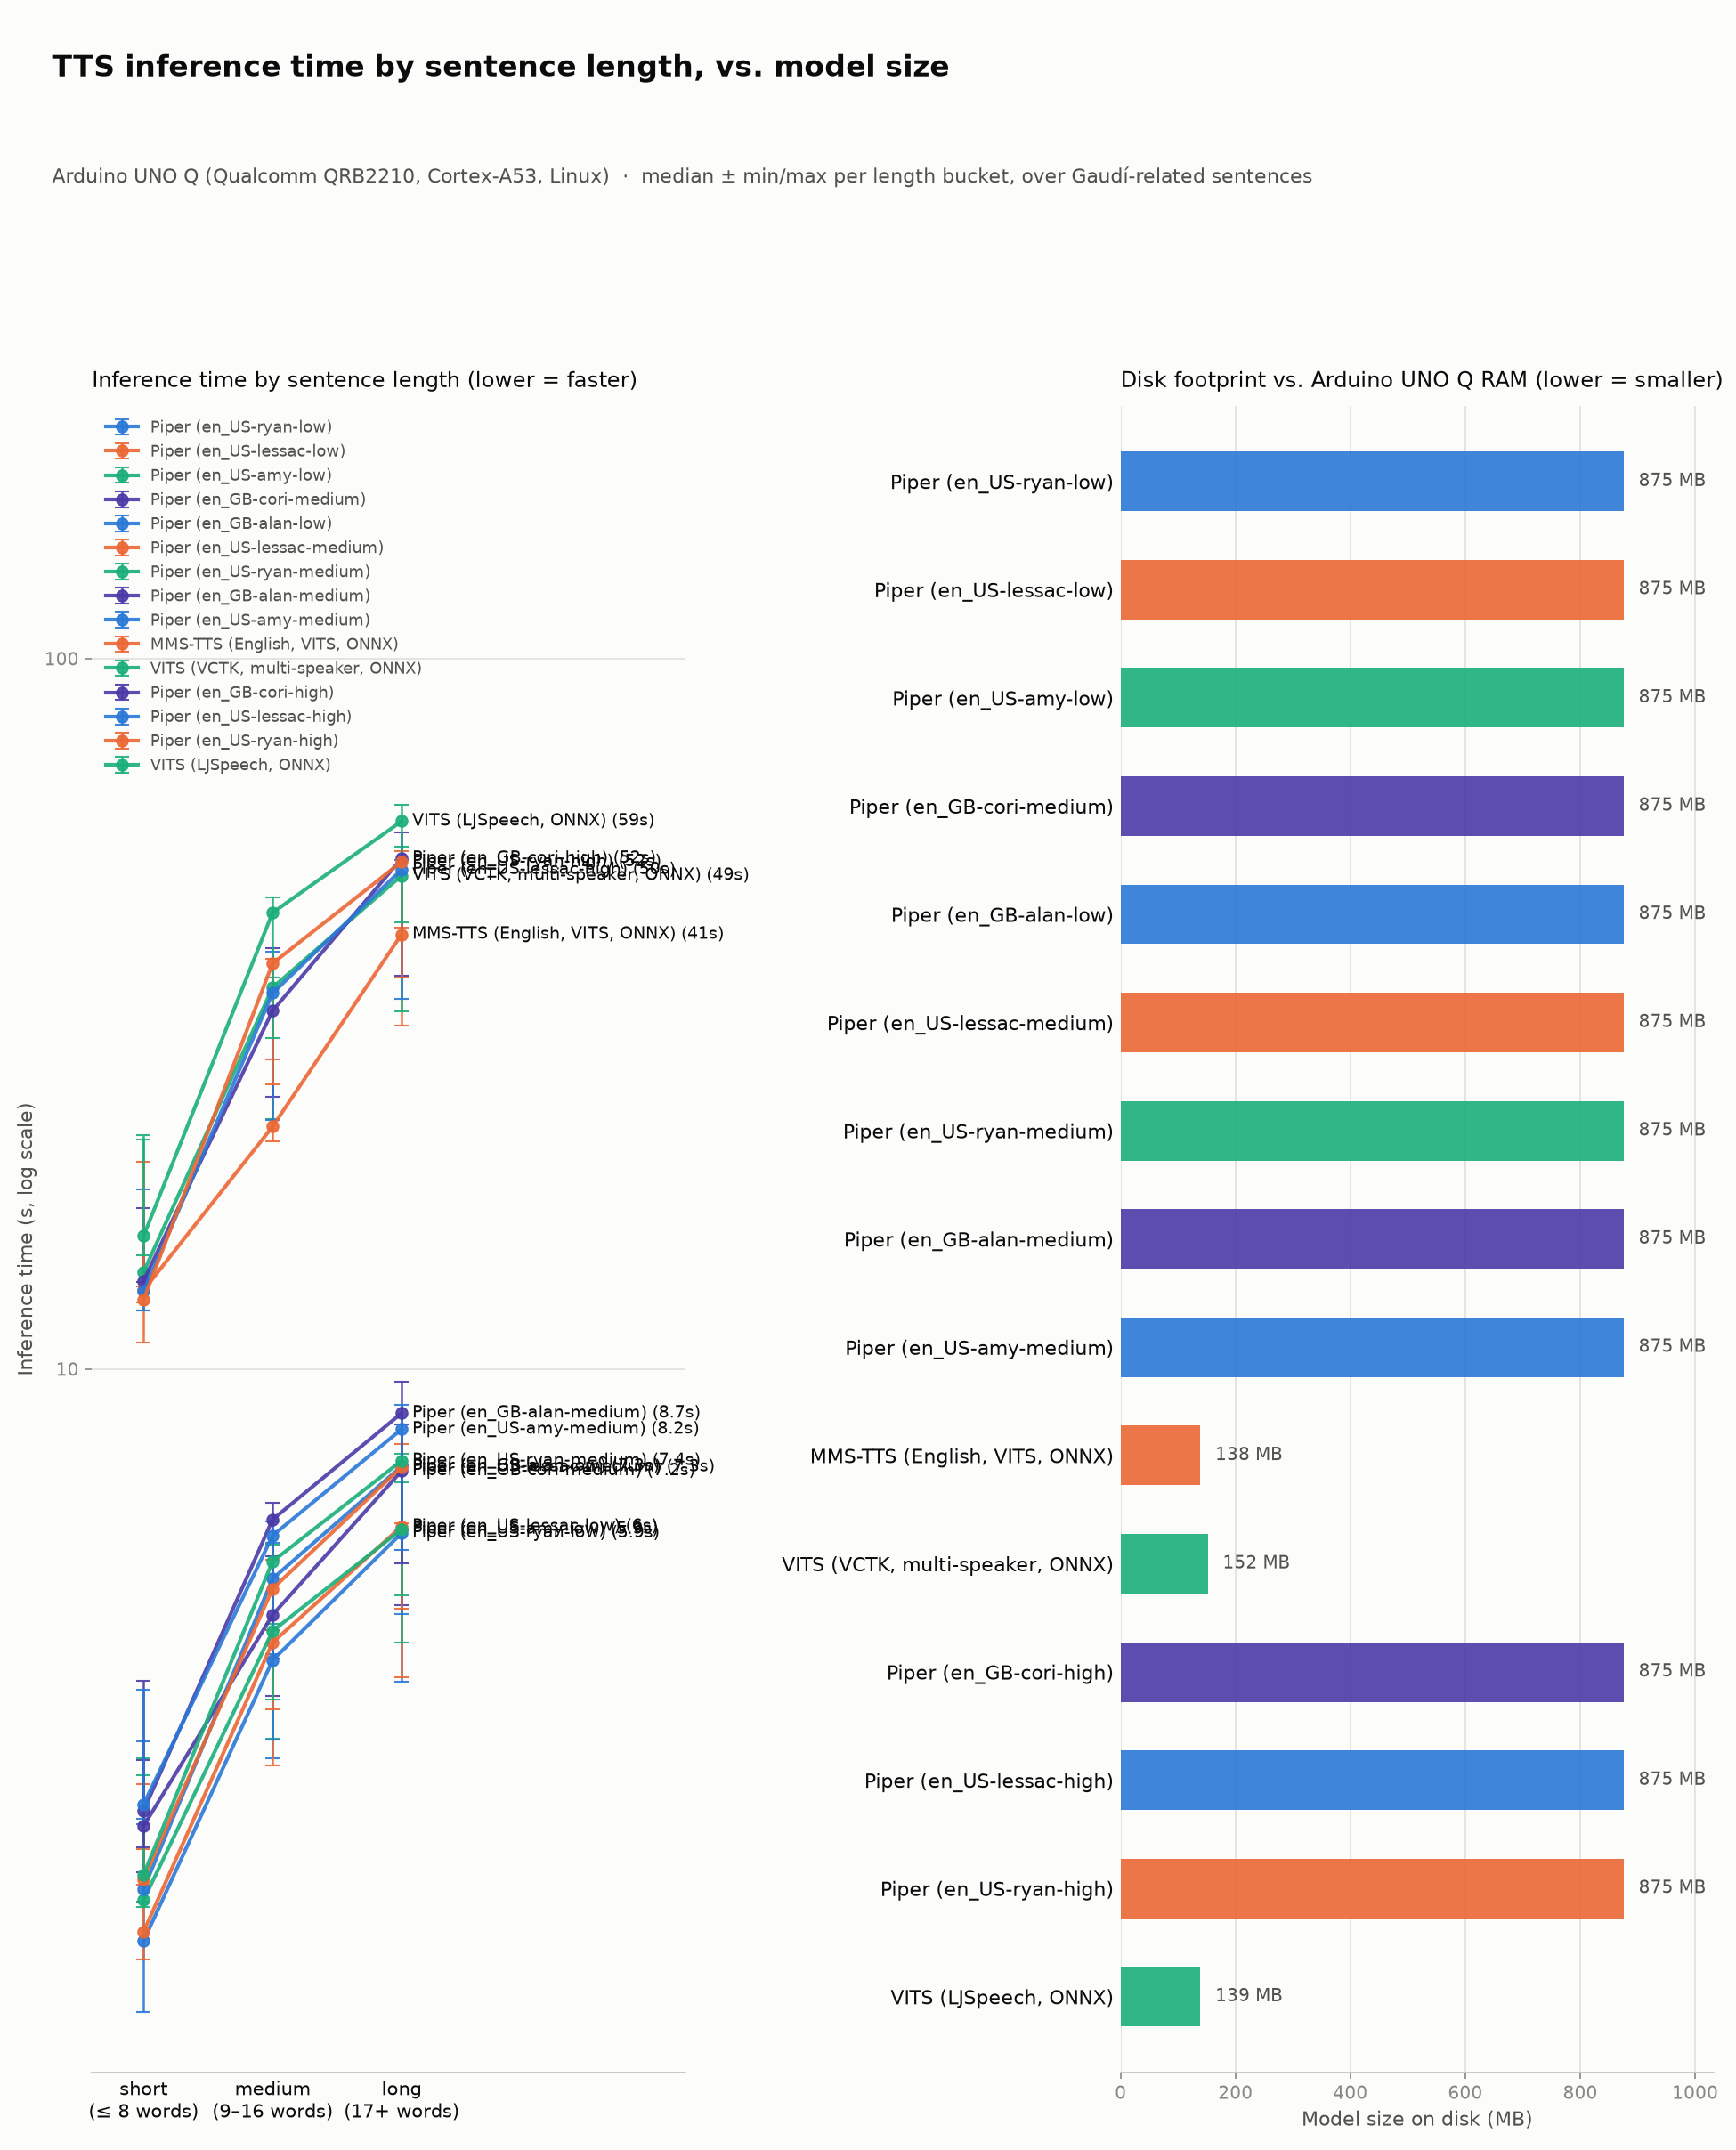
\includegraphics[width=\textwidth]{../benchmark/tts/results/comparison.png}
\caption{Median inference time with min/max whiskers per sentence-length
bucket, alongside on-disk model size, generated by \texttt{visualize.py} from
the same results file as Table~\ref{tab:tts}.}
\end{figure}

\subsubsection{Reading the results}

Table~\ref{tab:tts} separates the field cleanly into three groups.

\begin{itemize}
  \item \textbf{The VITS exports are unusable here.} RTF $\approx 3.8$ means
        roughly four seconds of compute per second of speech. A 20-second
        answer would take over a minute to synthesise.
  \item \textbf{Piper ``high'' voices are equally unusable}, and for the same
        reason --- RTF $\approx 5.2$--$5.3$, \emph{worse} than the VITS models
        despite Piper's much lighter runtime. The quality tier, not the
        framework, is what blows the budget.
  \item \textbf{Piper low and medium clear the bar with room to spare.} Every
        low voice lands at RTF $\approx 0.61$--$0.64$ and every medium voice at
        $\approx 0.75$--$0.81$. A medium voice synthesises a short sentence in
        about \SI{2}{\second} and a long one in about \SI{8}{\second}, while
        producing more audio than that in playback time --- which is what makes
        sentence-level streaming (\S\ref{sec:latency}) work: playback of
        sentence $N$ outlasts synthesis of sentence $N+1$, so the audio never
        stalls.
\end{itemize}

The gap between low and medium is around \SI{25}{\percent} of compute for a
clearly better voice, which is worth paying given the headroom.

\paragraph{Selected.} Two Piper medium voices ship on the device, mapped to
guide personalities:

\begin{center}
\begin{tabular}{lll}
\toprule
\textbf{Personality} & \textbf{Style} & \textbf{Voice} \\
\midrule
A --- Artistic  & Evocative, metaphorical & \texttt{en\_US-libritts\_r-medium} \\
B --- Technical & Architectural, precise  & \texttt{en\_GB-semaine-medium} (Spike) \\
C --- Child     & Simple, fun, story-led  & \texttt{en\_GB-semaine-medium} (Prudence) \\
\bottomrule
\end{tabular}
\end{center}

% ---------------------------------------------------------------------------
\subsection{End-to-end latency}
\label{sec:latency}
% ---------------------------------------------------------------------------

\texttt{python/benchmark.py} on the device measures the stages in isolation and
then reports the figure that actually matters.

\paragraph{Why the serial sum is the wrong number.} Adding up every stage
measured in isolation gives an upper bound, not a latency, because the pipeline
deliberately does not run them in sequence: vision happens at photo time,
prefill overlaps with recording, and Piper synthesises while
\texttt{llama.cpp} is still decoding.

The benchmark therefore reports \textbf{time to first audio} --- from the
moment the visitor stops speaking to the first word they hear. It counts only
the stages still on that path, each with the figure that applies there: STT in
full, the \emph{warm} prefill rather than the cold one, decode only as far as
the first complete sentence, and one sentence of Piper rather than the whole
answer. Any stage that could not be measured is named and the total flagged as
an underestimate, rather than being silently dropped. It excludes the
\texttt{aplay} spawn and Bridge RPC round-trips, which the harness does not
exercise, so the board is somewhat slower than the printed figure.

\paragraph{The three optimisations.}

\begin{enumerate}
  \item \textbf{Asynchronous prefill overlap.} Once a photo is confirmed, the
        static prompt prefix --- system instructions plus the monument's fact
        sheet --- is prefilled into the SLM KV-cache on a background thread
        while the visitor is still speaking. When recording ends, only the new
        user question needs prefilling. The prefix cache is additionally
        persisted to disk: \texttt{prewarm\_cache.py} computes it once per
        element ($\approx$\SI{30}{\second} each, $\approx$12 minutes for all
        24), so no visitor ever sits through a cold $\approx$\SI{30}{\second}
        prefill.
  \item \textbf{RMS silence detection with cropping.} Recording ends by itself
        once the visitor stops talking ($\approx$\SI{1.5}{\second} of silence),
        and the trailing and leading silence is cropped before the samples
        reach Whisper. This is not cosmetic: Whisper's encoder pads every
        window to a fixed length, so room tone between the last word and the
        stop is encoded at exactly the same price as speech. Cropping removes
        that cost from the critical path entirely. Thresholds adapt to the
        noise floor measured at the start of each recording; in a room too loud
        to judge, detection backs off and the physical button stops the
        recording as before.
  \item \textbf{Sentence-level streaming to TTS.} Rather than waiting for the
        full generation (60$+$ tokens), tokens are emitted sentence by
        sentence. Piper synthesises sentence $N$ while the SLM decodes sentence
        $N+1$. Given the Piper medium RTF of $\approx 0.8$ measured above, the
        synthesis pipeline stays comfortably ahead of playback.
\end{enumerate}

Together these move the perceived latency from ``sum of all four stages'' to
``STT $+$ warm prefill $+$ one sentence of decode $+$ one sentence of Piper''.

% ===========================================================================
\section{Bill of materials}
% ===========================================================================

\subsection{Arduino components}

Prices are Arduino Store (EU) list prices, VAT included, retrieved
13 September 2026 from \url{https://store.arduino.cc}. Product codes are given
where available.

\begin{table}[h]
\centering
\caption{Arduino components. The three Modulino modules are the ones this
project actually requires.}
\small\begin{tabular}{llrp{5.1cm}r}
\toprule
\textbf{Component} & \textbf{Code} & \textbf{Qty} & \textbf{Role in Cultura Viva} & \textbf{Price} \\
\midrule
Arduino UNO Q 4GB & --- & 1 & MCU $+$ Linux MPU, the whole system & \EUR{82.90} \\
\midrule
\multicolumn{5}{l}{\emph{Modulino modules (I\textsuperscript{2}C, Qwiic / Wire1)}} \\
Modulino Buttons & ABX00110 & 1 & Guide personality select A/B/C $+$ LEDs & \EUR{8.50} \\
Modulino Knob    & ABX00107 & 1 & Live headphone volume 0--100\,\% & \EUR{9.00} \\
Modulino Buzzer  & ABX00108 & 1 & Shutter click, confirmations, alerts & \EUR{7.30} \\
\midrule
Qwiic Cables Bundle & --- & 1 & Chains the Modulinos to the Wire1 port & \EUR{10.60} \\
\midrule
\multicolumn{4}{r}{\textbf{Modulino subtotal}} & \textbf{\EUR{24.80}} \\
\multicolumn{4}{r}{\textbf{Arduino subtotal}} & \textbf{\EUR{118.30}} \\
\bottomrule
\end{tabular}
\end{table}

\paragraph{Note on availability.} At the time of retrieval the Modulino Knob
(ABX00107) was listed as \emph{sold out} on the Arduino EU store. Its price is
as listed.

\paragraph{Note on the board variant.} The UNO Q also exists in a 2\,GB /
16\,GB variant at a lower price. All measurements in this report were taken on
the 4\,GB board (\SI{3667}{\mega\byte} detected). The 2\,GB variant would run
the pipeline only with the Qwen 2.5 0.5B fallback SLM, since the 1.5B model's
$\approx$\SI{1.45}{\giga\byte} working set leaves no room.

\subsection{Third-party components}

\begin{table}[h]
\centering
\caption{Non-Arduino components. \emph{These prices are indicative street
prices and were not verified against a single named vendor at the time of
writing --- replace with your actual purchase prices before publishing.}}
\small\begin{tabular}{llrp{5.1cm}r}
\toprule
\textbf{Component} & \textbf{Interface} & \textbf{Qty} & \textbf{Role} & \textbf{Price} \\
\midrule
ST7735S LCD, 1.8\,\textquotedbl{} 128$\times$160 & SPI & 1 & Live view, minimap, UI & \tbd \\
Logitech Brio 105 webcam & USB 2.0 & 1 & 1080p capture $+$ microphone & \tbd \\
NEO-6M GPS module & Serial1 @ 9600 & 1 & Monument proximity detection & \tbd \\
Mode switch (SPDT) & Digital D6 & 1 & Camera / map mode & \tbd \\
Push button & Digital D7 & 1 & Shutter / record / cancel & \tbd \\
Headphones or speaker & 3.5\,mm jack & 1 & Spoken answer output & \tbd \\
Jumper wires, carrier board & --- & --- & Assembly & \tbd \\
\midrule
\multicolumn{4}{r}{\textbf{Third-party subtotal}} & \tbd \\
\bottomrule
\end{tabular}
\end{table}

\subsection{Software cost}

Zero. Every model in the pipeline is open-weights and runs locally: the vision
backbones (\texttt{google/mobilenet\_v2\_1.0\_224},
\texttt{google/vit-base-patch16-224}), Whisper Base via faster-whisper,
Qwen 2.5 1.5B Instruct at \texttt{Q4\_K\_M}, and the Piper voices from
\texttt{rhasspy/piper-voices}. There are no inference API calls and no
per-visitor marginal cost. The Ragas judge used during evaluation
(\texttt{qwen2.5:7b} through Ollama) also runs locally and is a development-time
dependency only --- it never ships to the device.

% ===========================================================================
\section{Summary of selections}
% ===========================================================================

\begin{table}[h]
\centering
\caption{What the benchmarks selected, and on what grounds.}
\begin{tabular}{p{1.1cm}p{4.4cm}p{7.4cm}}
\toprule
\textbf{Stage} & \textbf{Selected} & \textbf{Decided on} \\
\midrule
Vision & Per-monument ONNX classifiers, $224\times224$, with entropy $+$
  confidence OOD gate & Accuracy / macro-F1 per monument; OOD rejection is a
  hard requirement, not a nicety \\
STT & faster-whisper \texttt{base.en}, INT8, 4 threads, greedy & 16.4\,\% WER
  but 96.1\,\% keyword accuracy --- proper nouns drive retrieval \\
SLM & Qwen 2.5 1.5B Instruct \texttt{Q4\_K\_M}
  (0.5B fallback for the 2\,GB board) & Answer quality and memory headroom;
  latency did not discriminate between candidates \\
TTS & Piper medium voices, per personality & RTF $\approx 0.8$ on the board,
  which is what makes sentence-level streaming viable \\
\bottomrule
\end{tabular}
\end{table}

% ===========================================================================
\section{Open items}
% ===========================================================================

The following numbers are referenced in this report but are not currently
exported into the repository, and appear above as \tbd:

\begin{enumerate}
  \item \textbf{Vision accuracy / macro-F1} for the 8
        $(\text{monument}, \text{backbone})$ runs
        (Table~\ref{tab:vision-results}). Logged to the Weights \& Biases
        project \texttt{cultura-viva}; \texttt{vision/outputs/} is gitignored.
  \item \textbf{Ragas scores} for the 5 SLM candidates.
        \texttt{eval/results/} is not checked in; regenerate with
        \texttt{uv run python main.py benchmark}.
  \item \textbf{STT results for whisper.cpp, Vosk and sherpa-onnx.} Only
        \texttt{faster-whisper:base.en} is present in
        \texttt{results\_computer/summary.json}.
  \item \textbf{Third-party component prices.}
  \item \textbf{Measured time-to-first-audio} from a board run of
        \texttt{python/benchmark.py --json}.
\end{enumerate}

\end{document}
